% Arquivo LaTeX de exemplo de dissertação/tese a ser apresentada à CPG do IME-USP
%
% Criação: Jesús P. Mena-Chalco
% Revisão: Fabio Kon e Paulo Feofiloff
% Adaptação para UTF8, biblatex e outras melhorias: Nelson Lago
%
% Except where otherwise indicated, these files are distributed under
% the MIT Licence. The example text, which includes the tutorial and
% examples as well as the explanatory comments in the source, are
% available under the Creative Commons Attribution International
% Licence, v4.0 (CC-BY 4.0) - https://creativecommons.org/licenses/by/4.0/


%%%%%%%%%%%%%%%%%%%%%%%%%%%%%%%%%%%%%%%%%%%%%%%%%%%%%%%%%%%%%%%%%%%%%%%%%%%%%%%%
%%%%%%%%%%%%%%%%%%%%%%%%%%%%%%% PREÂMBULO LaTeX %%%%%%%%%%%%%%%%%%%%%%%%%%%%%%%%
%%%%%%%%%%%%%%%%%%%%%%%%%%%%%%%%%%%%%%%%%%%%%%%%%%%%%%%%%%%%%%%%%%%%%%%%%%%%%%%%

% A opção twoside (frente-e-verso) significa que a aparência das páginas pares
% e ímpares pode ser diferente. Por exemplo, as margens podem ser diferentes ou
% os números de página podem aparecer à direita ou à esquerda alternadamente.
% Mas nada impede que você crie um documento "só frente" e, ao imprimir, faça
% a impressão frente-e-verso.
%
% Aqui também definimos a língua padrão do documento (a última da lista) e
% línguas adicionais. Para teses do IME, no mínimo português e inglês são
% obrigatórios, porque independentemente da língua principal do texto é
% preciso fornecer o resumo nessas duas línguas. LaTeX aceita alguns nomes
% diferentes para a língua portuguesa; dentre as opções, prefira sempre
% "brazilian" para português brasileiro e "portuguese" para português europeu.
%\documentclass[a4paper,12pt,twoside,brazilian,english]{book}
\documentclass[a4paper,12pt,twoside,english,brazilian]{book}

% O preâmbulo de um documento LaTeX pode ser razoavelmente longo. Neste
% modelo, optamos por reduzi-lo, colocando praticamente tudo do preâmbulo
% nas packages "imegoodies" e "imelooks".
%
% imegoodies carrega diversas packages muito úteis e populares (algumas
% são praticamente obrigatórias, como amsmath, babel, array etc.). É
% uma boa ideia usá-la com outros documentos também. Ela inclui vários
% comentários explicativos e dicas de uso; não tenha medo de alterá-la
% conforme a necessidade.
%
% imelooks carrega algumas packages e configurações que definem a
% aparência do documento; você também pode querer usá-la (ou partes
% dela) com outros documentos para obter as mesmas fontes, margens
% etc. Tal como "imegoodies", pode valer a pena ler os comentários
% e fazer modificações nessa package. Com a opção "thesis", imelooks
% também define os comandos para capa, folha de rosto etc.
\usepackage{imegoodies}
\usepackage[thesis]{imelooks}

%\nocolorlinks % para impressão em P&B

% Diretórios onde estão as figuras; com isso, não é necessário (mas
% é permitido) colocar o caminho completo em \includegraphics. Note
% que a extensão nunca é necessária (mas é permitida), ou seja, o
% resultado é o mesmo com "\includegraphics{figuras/foto.jpeg}",
% "\includegraphics{foto.jpeg}", "\includegraphics{figuras/foto}"
% ou "\includegraphics{foto}".
\graphicspath{{figuras/},{fig/},{logos/},{img/},{images/},{imagens/}}

% Comandos rápidos para mudar de língua:
% \en -> muda para o inglês
% \br -> muda para o português
% \texten{blah} -> o texto "blah" é em inglês
% \textbr{blah} -> o texto "blah" é em português
\babeltags{br = brazilian, en = english}


%%%%%%%%%%%%%%%%%%%%%%%%%%%%%%%%%%%%%%%%%%%%%%%%%%%%%%%%%%%%%%%%%%%%%%%%%%%%%%%%
%%%%%%%%%%%%%%%%%%%%%%%%%%%%%%%%%% METADADOS %%%%%%%%%%%%%%%%%%%%%%%%%%%%%%%%%%%
%%%%%%%%%%%%%%%%%%%%%%%%%%%%%%%%%%%%%%%%%%%%%%%%%%%%%%%%%%%%%%%%%%%%%%%%%%%%%%%%

% O arquivo com os dados bibliográficos para biblatex; você pode usar
% este comando mais de uma vez para acrescentar múltiplos arquivos
\addbibresource{bibliografia.bib}

% Este comando permite acrescentar itens à lista de referências sem incluir
% uma referência de fato no texto (pode ser usado em qualquer lugar do texto)
%\nocite{bronevetsky02,schmidt03:MSc, FSF:GNU-GPL, CORBA:spec, MenaChalco08}
% Com este comando, todos os itens do arquivo .bib são incluídos na lista
% de referências
%\nocite{*}

% É possível definir como determinadas palavras podem (ou não) ser
% hifenizadas; no entanto, a hifenização automática geralmente funciona bem
\babelhyphenation{documentclass latexmk soft-ware clsguide} % todas as línguas
\babelhyphenation[brazilian]{Fu-la-no}
\babelhyphenation[english]{what-ever}

% Estes comandos definem o título e autoria do trabalho e devem sempre ser
% definidos, pois além de serem utilizados para criar a capa, também são
% armazenados nos metadados do PDF. O subtítulo é opcional.
\title{Árvores binárias de busca e a Conjectura da Otimalidade Dinâmica}
\translatedtitle{Binary search trees and the Dynamic Optimality Conjecture}

\author[masc]{Bruno Armond Braga}

\def\profa{Prof\kern.02em.\kern-.07emª\kern.07em}
\def\dra{Dr\kern-.04em.\kern-.11emª\kern.07em}

% Para TCCs, este comando define o supervisor
\orientador[fem]{\profa{} \dra{} Cristina Gomes Fernandes}

\banca{
  \profa{} \dra{} Fulana de Tal (orientadora) -- IME-USP [sem ponto final],
  % Em inglês, não há o "ª"
  %Prof. Dr. Fulana de Tal (advisor) -- IME-USP [sem ponto final],
  Prof. Dr. Ciclano de Tal -- IME-USP [sem ponto final],
  \profa{} \dra{} Convidada de Tal -- IMPA [sem ponto final],
}

% A página de rosto da versão para depósito (ou seja, a versão final
% antes da defesa) deve ser diferente da página de rosto da versão
% definitiva (ou seja, a versão final após a incorporação das sugestões
% da banca).
\tipotese{
  %mestrado,
  %doutorado,
  tcc,
  %definitiva, % É a versão para defesa ou a versão definitiva?
  %quali, % É qualificação?
  programa={Ciência da Computação},
}

\defesa{
  local={São Paulo},
  data=2024-08-10, % YYYY-MM-DD
}

% Se não houve bolsa, remova
%
% Norma sobre agradecimento por auxílios da FAPESP:
% https://fapesp.br/11789/referencia-ao-apoio-da-fapesp-em-todas-as-formas-de-divulgacao
%
% Norma sobre agradecimento por auxílios da CAPES (Portaria 206,
% de 4 de Setembro de 2018):
% https://www.in.gov.br/materia/-/asset_publisher/Kujrw0TZC2Mb/content/id/39729251/do1-2018-09-05-portaria-n-206-de-4-de-setembro-de-2018-39729135
%
%\apoio{O presente trabalho foi realizado com apoio da Coordenação
%      de Aperfeiçoamento\\ de Pessoal de Nível Superior -- Brasil
%      (CAPES) -- Código de Financiamento 001} % o código é sempre 001
%
%\apoio{This study was financed in part by the Coordenação de
%      Aperfeiçoamento\\ de Pessoal de Nível Superior -- Brasil
%      (CAPES) -- Finance Code 001} % o código é sempre 001
%
%\apoio{Durante o desenvolvimento deste trabalho, o autor recebeu\\
%      auxílio financeiro da FAPESP -- processo nº aaaa/nnnnn-d}
%
%\apoio{During the development if this work, the author received\\
%      financial support from FAPESP -- grant \#aaaa/nnnnn-d}
%\apoio{Durante o desenvolvimento deste trabalho o autor
%       recebeu auxílio financeiro da XXXX}

% A licença do seu trabalho. Use CC-BY, CC-BY-NC, CC-BY-ND, CC-BY-SA,
% CC-BY-NC-SA ou CC-BY-NC-ND para escolher a licença Creative Commons
% correspondente (o sistema insere automaticamente o texto da licença).
% Se quiser estabelecer regras diferentes para o uso de seu trabalho,
% converse com seu orientador e coloque o texto da licença aqui, mas
% observe que apenas TCCs sob alguma licença Creative Commons serão
% acrescentados ao BDTA. Se você tem alguma intenção de publicar o
% trabalho comercialmente no futuro, sugerimos a licença CC-BY-NC-ND.
%
%\direitos{CC-BY-NC-ND}
%
%\direitos{Autorizo a reprodução e divulgação total ou parcial deste
%          trabalho, por qualquer meio convencional ou eletrônico,
%          para fins de estudo e pesquisa, desde que citada a fonte.}
%
%\direitos{I authorize the complete or partial reproduction and disclosure
%          of this work by any conventional or electronic means for study
%          and research purposes, provided that the source is acknowledged.}
%
\direitos{CC-BY}

% Para gerar a ficha catalográfica, acesse https://fc.ime.usp.br/,
% preencha o formulário e escolha a opção "Gerar Código LaTeX".
% Basta copiar e colar o resultado aqui.
\fichacatalografica{}


%%%%%%%%%%%%%%%%%%%%%%%%%%%%%%%%%%%%%%%%%%%%%%%%%%%%%%%%%%%%%%%%%%%%%%%%%%%%%%%%
%%%%%%%%%%%%%%%%%%%%%%% AQUI COMEÇA O CONTEÚDO DE FATO %%%%%%%%%%%%%%%%%%%%%%%%%
%%%%%%%%%%%%%%%%%%%%%%%%%%%%%%%%%%%%%%%%%%%%%%%%%%%%%%%%%%%%%%%%%%%%%%%%%%%%%%%%

\newtheorem{theorem}{Teorema}[chapter]
\newtheorem{lemma}[theorem]{Lema}

\begin{document}

%%%%%%%%%%%%%%%%%%%%%%%%%%% CAPA E PÁGINAS INICIAIS %%%%%%%%%%%%%%%%%%%%%%%%%%%%

% Aqui começa o conteúdo inicial que aparece antes do capítulo 1, ou seja,
% página de rosto, resumo, sumário etc. O comando frontmatter faz números
% de página aparecem em algarismos romanos ao invés de arábicos e
% desabilita a contagem de capítulos.
\frontmatter

\pagestyle{plain}

\onehalfspacing % Espaçamento 1,5 na capa e páginas iniciais

\maketitle % capa e folha de rosto

%%%%%%%%%%%%%%%% DEDICATÓRIA, AGRADECIMENTOS, RESUMO/ABSTRACT %%%%%%%%%%%%%%%%%%

\begin{dedicatoria}
Esta seção é opcional e fica numa página separada; ela pode ser usada para
uma dedicatória ou epígrafe.
\end{dedicatoria}

% Reinicia o contador de páginas (a próxima página recebe o número "i") para
% que a página da dedicatória não seja contada.
\pagenumbering{roman}

% Agradecimentos:
% Se o candidato não quer fazer agradecimentos, deve simplesmente eliminar
% esta página. A epígrafe, obviamente, é opcional; é possível colocar
% epígrafes em todos os capítulos. O comando "\chapter*" faz esta seção
% não ser incluída no sumário.
\chapter*{Agradecimentos}
\epigrafe{Do. Or do not. There is no try.}{Mestre Yoda}

Texto texto texto texto texto texto texto texto texto texto texto texto texto
texto texto texto texto texto texto texto texto texto texto texto texto texto
texto texto texto texto texto texto texto texto texto texto texto texto texto
texto texto texto texto. Texto opcional.

%!TeX root=../tese.tex
%("dica" para o editor de texto: este arquivo é parte de um documento maior)
% para saber mais: https://tex.stackexchange.com/q/78101

% As palavras-chave são obrigatórias, em português e em inglês, e devem ser
% definidas antes do resumo/abstract. Acrescente quantas forem necessárias.
\palavraschave{Palavra-chave1, Palavra-chave2, Palavra-chave3}

\keywords{Keyword1,Keyword2,Keyword3}

% O resumo é obrigatório, em português e inglês. Estes comandos também
% geram automaticamente a referência para o próprio documento, conforme
% as normas sugeridas da USP.
\resumo{
Elemento obrigatório, constituído de uma sequência de frases concisas e
objetivas, em forma de texto. Deve apresentar os objetivos, métodos empregados,
resultados e conclusões. O resumo deve ser redigido em parágrafo único, conter
no máximo 500 palavras e ser seguido dos termos representativos do conteúdo do
trabalho (palavras-chave). Deve ser precedido da referência do documento.
Texto texto texto texto texto texto texto texto texto texto texto texto texto
texto texto texto texto texto texto texto texto texto texto texto texto texto
texto texto texto texto texto texto texto texto texto texto texto texto texto
texto texto texto texto texto texto texto texto texto texto texto texto texto
texto texto texto texto texto texto texto texto texto texto texto texto texto
texto texto texto texto texto texto texto texto.
Texto texto texto texto texto texto texto texto texto texto texto texto texto
texto texto texto texto texto texto texto texto texto texto texto texto texto
texto texto texto texto texto texto texto texto texto texto texto texto texto
texto texto texto texto texto texto texto texto texto texto texto texto texto
texto texto.
}

\abstract{
Elemento obrigatório, elaborado com as mesmas características do resumo em
língua portuguesa. De acordo com o Regimento da Pós-Graduação da USP (Artigo
99), deve ser redigido em inglês para fins de divulgação. É uma boa ideia usar
o sítio \url{www.grammarly.com} na preparação de textos em inglês.
Text text text text text text text text text text text text text text text text
text text text text text text text text text text text text text text text text
text text text text text text text text text text text text text text text text
text text text text text text text text text text text text.
Text text text text text text text text text text text text text text text text
text text text text text text text text text text text text text text text text
text text text.
}



%%%%%%%%%%%%%%%%%%%%%%%%%%% LISTAS DE FIGURAS ETC. %%%%%%%%%%%%%%%%%%%%%%%%%%%%%

% Como as listas que se seguem podem não incluir uma quebra de página
% obrigatória, inserimos uma quebra manualmente aqui.
%\cleardoublepage

% Todas as listas são opcionais; Usando "\chapter*" elas não são incluídas
% no sumário. As listas geradas automaticamente também não são incluídas por
% conta das opções "notlot" e "notlof" que usamos para a package tocbibind.

% Normalmente, "\chapter*" faz o novo capítulo iniciar em uma nova página, e as
% listas geradas automaticamente também por padrão ficam em páginas separadas.
% Como cada uma destas listas é muito curta, não faz muito sentido fazer isso
% aqui, então usamos este comando para desabilitar essas quebras de página.
% Se você preferir, comente as linhas com esse comando e des-comente as linhas
% sem ele para criar as listas em páginas separadas. Observe que você também
% pode inserir quebras de página manualmente (com \clearpage, veja o exemplo
% mais abaixo).
%\newcommand\disablenewpage[1]{{\let\clearpage\par\let\cleardoublepage\par #1}}
\newcommand{\tdots}{{\,.\,.\,}}

% Nestas listas, é melhor usar "raggedbottom" (veja basics.tex). Colocamos
% a opção correspondente e as listas dentro de um grupo para ativar
% raggedbottom apenas temporariamente.
%\bgroup
%\raggedbottom

%%%%% Listas criadas manualmente

%\chapter*{Lista de abreviaturas}
%\disablenewpage{\chapter*{Lista de abreviaturas}}

%\begin{tabular}{rl}
%   CFT & Transformada contínua de Fourier (\emph{Continuous Fourier Transform})\\
%   DFT & Transformada discreta de Fourier (\emph{Discrete Fourier Transform})\\
%  EIIP & Potencial de interação elétron-íon (\emph{Electron-Ion Interaction Potentials})\\
%  STFT & Transformada de Fourier de tempo reduzido (\emph{Short-Time Fourier Transform})\\
%  ABNT & Associação Brasileira de Normas Técnicas\\
%   URL & Localizador Uniforme de Recursos (\emph{Uniform Resource Locator})\\
%   IME & Instituto de Matemática e Estatística\\
%   USP & Universidade de São Paulo
%\end{tabular}

%\chapter*{Lista de símbolos}
%\disablenewpage{\chapter*{Lista de símbolos}}

%\begin{tabular}{rl}
%  $\omega$ & Frequência angular\\
%    $\psi$ & Função de análise \emph{wavelet}\\
%    $\Psi$ & Transformada de Fourier de $\psi$\\
%\end{tabular}

% Quebra de página manual
%\clearpage

%%%%% Listas criadas automaticamente

% Você pode escolher se quer ou não permitir a quebra de página
%\listoffigures
%\disablenewpage{\listoffigures}

% Você pode escolher se quer ou não permitir a quebra de página
%\listoftables
%\disablenewpage{\listoftables}

% Esta lista é criada "automaticamente" pela package float quando
% definimos o novo tipo de float "program" (em utils.tex)
% Você pode escolher se quer ou não permitir a quebra de página
%\listof{program}{\programlistname}
%\disablenewpage{\listof{program}{\programlistname}}

% Sumário (obrigatório)
%\tableofcontents

%\egroup % Final de "raggedbottom"

% Referências indiretas ("x", veja "y") para o índice remissivo (opcionais,
% pois o índice é opcional). É comum colocar esses itens no final do documento,
% junto com o comando \printindex, mas em alguns casos isso torna necessário
% executar texindy (ou makeindex) mais de uma vez, então colocar aqui é melhor.
%\index{Inglês|see{Língua estrangeira}}
%\index{Figuras|see{Floats}}
%\index{Tabelas|see{Floats}}
%\index{Código-fonte|see{Floats}}
%\index{Subcaptions|see{Subfiguras}}
%\index{Sublegendas|see{Subfiguras}}
%\index{Equações|see{Modo matemático}}
%\index{Fórmulas|see{Modo matemático}}
%\index{Rodapé, notas|see{Notas de rodapé}}
%\index{Captions|see{Legendas}}
%\index{Versão original|see{Tese/Dissertação, versões}}
%\index{Versão corrigida|see{Tese/Dissertação, versões}}
%\index{Palavras estrangeiras|see{Língua estrangeira}}
%\index{Floats!Algoritmo|see{Floats, ordem}}


%%%%%%%%%%%%%%%%%%%%%%%%%%%%%%%% CAPÍTULOS %%%%%%%%%%%%%%%%%%%%%%%%%%%%%%%%%%%%%

% Aqui vai o conteúdo principal do trabalho, ou seja, os capítulos que compõem
% a dissertação/tese. O comando mainmatter reinicia a contagem de páginas,
% modifica a numeração para números arábicos e ativa a contagem de capítulos.
\mainmatter

\pagestyle{mainmatter}

% Espaçamento simples
\singlespacing

% A introdução não tem número de capítulo, então os cabeçalhos também não
\pagestyle{unnumberedchapter}
%!TeX root=../tese.tex
%("dica" para o editor de texto: este arquivo é parte de um documento maior)
% para saber mais: https://tex.stackexchange.com/q/78101/183146

%% ------------------------------------------------------------------------- %%
\chapter{Introdução}
\label{cap:introducao}

Árvores Binárias de Busca (ABBs) são estruturas de dados que armazenam um conjunto de chaves de um universo estático, que possui uma ordem total, e dão suporte a buscas neste conjunto. Denotaremos por $n$ o número de elementos do conjunto armazenado na ABB considerada.

Estas estruturas são fundamentais na ciência da computação e possuem as mais diversas finalidades. Nesse projeto iremos estudar a chamada Conjectura da Otimalidade Dinâmica, interpretações geométricas de algoritmos de busca em ABBs e suas delimitações associadas. Também serão estudadas as árvores splay e as árvores tango.

Adaptando a definição dada por Sedgewick e Wayne \cite{Sedgewick}, \textit{árvore binária de busca} é uma árvore binária onde cada nó possui uma chave comparável e possivelmente um valor associado. Além disso, os nós satisfazem a restrição de que a chave em qualquer nó é maior do que as chaves em todos os nós na subárvore esquerda desse nó e menor do que as chaves em todos os nós na subárvore direita desse nó.

As ABBs também possuem um atributo \textit{raiz} que aponta para o nó raiz ou possui valor \textit{nulo}, caso a árvore esteja vazia.

\textit{Rotações} são operações que trocam dois nós, pai-filho, entre si enquanto mantém a restrição vista acima. Veja a Figura~\ref{fig:imagem}. Essa operação é fundamental para garantir performance em alguns algoritmos de ABBs e é muito utilizada para controlar a altura das árvores.


% Arrumar figura!!
\begin{figure}[h]
    \centering
    \includegraphics{imagens/zig2.pdf}
    \caption{Esquema de rotações.}
    \label{fig:imagem}
\end{figure}

No contexto da Conjectura da Otimalidade Dinâmica, apenas serão consideradas buscas bem sucedidas, que chamaremos de \textit{acessos}, e não são consideradas inserções ou remoções no conjunto armazenado. No modelo de computação adotado, um algoritmo de busca em uma ABB, para fazer o acesso a uma chave, mantém um único ponteiro. Chamamos de \textit{nó corrente} o nó apontado por esse ponteiro. 

No início da execução do acesso, o ponteiro aponta para a raiz da árvore e, após uma sequência de operações, deve encontrar o nó que armazena a chave procurada. As operações chamadas de \textit{primitivas} são:
\begin{enumerate}
    \item Mover o ponteiro para o filho esquerdo do nó corrente.
    \item Mover o ponteiro para o filho direito do nó corrente.
    \item Mover o ponteiro para o pai do nó corrente.
    \item Fazer uma rotação que troca a posição do nó corrente e do seu pai.
\end{enumerate}

O algoritmo tradicional de busca em ABB não executa a operação primitiva 4. Ele inicia a execução de um acesso na raiz e desce para o filho apropriado até alcançar a chave procurada. No modelo de computação adotado, todas essas operações possuem custo unitário.

Em geral, durante a execução de um acesso, uma série de nós distintos são apontados pelo ponteiro do algoritmo de busca. Ao fim da execução de uma busca bem sucedida, o nó corrente é o nó procurado. Assim, dizemos que o nó procurado foi \textit{acessado} e que todos os nós que foram apontados pelo ponteiro durante a busca foram \textit{visitados}. O nó acessado também é considerado um nó visitado.

O pior caso acontece quando a chave procurada está em um nó folha mais profundo. Nesse caso o algoritmo tem que passar por toda a altura da árvore até chegar a essa folha. Assim o custo do pior caso é proporcional à altura da árvore, que pode ser em princípio linear em $n$.

Com intuito de mitigar o custo do pior caso, algumas ABBs estrategicamente utilizam da operação primitiva 4 (rotação) para balancear o tamanho das subárvores e assim diminuir a altura da árvore. Um exemplo famoso, sobre o qual daremos mais detalhes à frente, é a árvore splay. Essa ABB executa rotações baseando-se na heurística ``move to front'' e assim balanceia a árvore durante as buscas. Essa árvore não utiliza armazenamento adicional para isso, ou seja, seus nós não têm campos extra.

O custo para executar um acesso nesse modelo está relacionado com o número de operações primitivas executadas até encontrar a chave procurada durante um acesso. 

No artigo de Demaine et al.~\cite{rotation_distance}, é demonstrada a seguinte propriedade sobre ABBs. É possível transformar qualquer ABB com $t$ nós em qualquer outra ABB com os mesmos $t$ nós com no máximo $2t - 6$ rotações. O número preciso não é tão relevante para a análise desse texto. O importante é notar que o número de rotações necessárias para transformar uma ABB $T$ com $t$ nós em uma ABB $T'$ com os mesmos $t$ nós disposta de qualquer outra maneira é $\Oh(t)$, ou seja, é linear no número de nós da ABB.

Por isso, podemos assumir que o número de rotações realizadas durante um acesso é linear no número de nós visitados, assim definiremos o custo para executar um acesso nesse modelo como o número de nós visitados durante esse acesso.

Como o conjunto armazenado nas ABBs que consideraremos não sofre alterações, podemos assumir que esse conjunto é \{1,2,\ldots,$n$\}.

ABBs \textit{online} são ABBs que apenas possuem informações sobre os acessos passados. Ou seja, se $X = (x_1, \ldots, x_m)$ é a sequência de acessos que serão feitos, onde cada $x_i \in \{1,2,\ldots,n\}$, ao acessar $x_{i}$, um algoritmo de busca online não tem conhecimento das chaves $x_{i+1},\ldots,x_{m}$, nem mesmo do valor de $m$. Em particular, muitas ABBs online possuem informações adicionais em cada nó que auxiliam o algoritmo de busca a decidir quando executar rotações durante a busca pelas chaves procuradas. Qualquer ABB online que usa $\Oh(1)$ palavras adicionais por nó possui tempo de execução dominado pelo número de operações primitivas.

Uma ABB é chamada de \textit{offline} se tem conhecimento da sequência $X$ de acessos antes de começar os acessos às chaves de $X$. Nesse contexto, o comportamento do algoritmo não depende unicamente do histórico de acessos passados, uma vez que o algoritmo possui conhecimento prévio de toda a sequência de chaves a serem acessadas.

Dada uma sequência $X$ de acessos, uma ABB é considerada \textit{ótima} se executa os acessos de $X$ com o menor custo possível. Podemos definir OPT$(X)$ como o número de nós visitados por uma ABB ótima para a sequência $X$. Em outras palavras, OPT$(X)$ é o número mínimo necessário de visitas a nós para uma ABB concluir todos os acessos de $X$. 

ABBs balanceadas estabelecem que OPT$(X)$ = $\Oh(m \log n)$, onde $n$ é o número de chaves armazenadas na árvore e $m$ é o comprimento de $X$. Como todo acesso tem custo maior ou igual a 1, então $\text{OPT}(X) \geq m$. Wilber \cite{lowerbound_wilber} provou que OPT$(X)$ = $\Theta$$(m \log n)$ para algumas classes de sequências $X$. 

% JÁ USEI ESSA FRASE!
Uma ABB online é \textit{dinamicamente ótima} se, para todas as sequências $X$, seu algoritmo de busca tem custo $\Oh$(OPT($X$)). De maneira mais geral, uma ABB online é \textit{$c$-competitiva} se executa todos os acessos da sequências $X$ suficientemente longas com custo no máximo $c$\,OPT($X$).

Todo esse estudo foi feito para tentar responder à pergunta: ``\textit{Existe uma ABB online dinamicamente ótima?}".

Uma das tentativas de responder tal pergunta foi a árvore splay de Sleator e Tarjan~\cite{selfadjustingbst}. Como já mencionamos, árvores splay são ABBs que seguem a heurística ``move to front". Mais precisamente, após cada acesso, a árvore se reestrutura de uma maneira particular, trazendo o nó da chave que foi acessada para a raiz da árvore.

Apesar de existirem muitas ABBs muito bem documentadas com tempo por busca logarítmico em $n$, essas estruturas normalmente não conseguem alcançar uma eficiência superior a isso independentemente da entrada. Padrões de acesso do mundo real muitas vezes possuem estruturas repetitivas, como por exemplo bancos de dados que recebem solicitações frequentes para um pequeno número de elementos de alto tráfego. Em alguns desses casos, é possível ter uma performance melhor que $\Theta(\log n)$ por acesso utilizando uma árvore splay, uma vez que essa eventualmente ficaria com as chaves mais acessadas mais próximas à raiz da árvore. 

Há uma conjectura não resolvida no artigo \cite{selfadjustingbst} que diz que as árvores splay são dinamicamente ótimas. Essa conjectura ficou conhecida como a Conjectura da Otimalidade Dinâmica.

A árvore conhecida que mais se aproxima de uma árvore ótima é a árvores tango~\cite{dynamicoptimality}. Tal estrutura é $\Oh(\lg \lg n)$-competitiva. Esta árvore, proposta por Demaine, Harmon, Iacono e Pătrașcu \cite{dynamicoptimality}, utiliza $\Oh(\lg \lg n)$ bits a mais por nó e o custo para determinar a próxima operação primitiva a ser executada é amortizadamente constante.

%Nas árvores tango, há a definição de \textit{filho preferido}. O \textit{filho preferido} de um nó é o filho direito se ele foi o nó mais recentemente acessado em comparação com o nó esquerdo, e caso contrário (incluindo o caso em que nenhum dos dois filhos foi acessado ainda), definimos o nó esquerdo como \textit{filho preferido}.

%Define-se então um \textit{caminho preferido} como um caminho maximal de um nó da ABB até a folha que passa apenas por \textit{filhos preferidos}. 

%Os caminhos preferidos particionam os nós da árvore. Nas árvores tango, os nós de cada caminho preferido são armazenados em uma ABB balanceada tendo como chave a profundidade do nó no caminho. Essas árvores auxiliares estão interligadas de uma maneira apropriada.

%Durante os \textit{acessos}, os \textit{filhos preferidos} podem ser alterados e isso provocará mudanças nas estruturas da árvores auxiliares para manter a estrutura da árvore tango coerentes com o comportamento descrito acima.

Nesse texto, abordaremos uma série de aspectos diferentes em relação a delimitações de custo em algoritmos de busca em ABBs e implementações visando o menor custo possível. No Capítulo 2, será discutido o problema de encontrar uma ABB estática de custo mínimo para uma determinada sequência de acessos. No Capítulo 3, abordaremos o funcionamento e o custo das operações das árvores splay e apresentaremos a Conjectura da Otimalidade Dinâmica. 
No Capítulo 4, examinaremos como tratar buscas em ABBs de maneira geométrica por meio de conjuntos arboreamente satisfeitos e será proposto um algoritmo offline guloso para encontrar conjuntos arboreamente satisfeitos para sequências de entradas. %e será apresentada uma análise de como transforma-lo em um algoritmo online. 
No Capítulo 5, ampliaremos a análise geométrica para desenvolver uma nova delimitação relacionada a retângulos independentes. O Capítulo 6 tratará das delimitações de Wilber e, por fim, no Capítulo 7 explicaremos como funcionam as árvores tango.
\pagestyle{mainmatter}
%!TeX root=../tese.tex
%("dica" para o editor de texto: este arquivo é parte de um documento maior)
% para saber mais: https://tex.stackexchange.com/q/78101/183146

%% ------------------------------------------------------------------------- %%
\chapter{Problema Estático}
\label{cap:problema-estatico}

Neste capítulo será apresentado a solução para encontrar uma árvore de busca binária com custo mínimo para um determinado 
%%!TeX root=../tese.tex
%("dica" para o editor de texto: este arquivo é parte de um documento maior)
% para saber mais: https://tex.stackexchange.com/q/78101/183146

%% ------------------------------------------------------------------------- %%
\chapter{Árvores splay}
\label{cap:arvores-splay}

Neste capítulo apresentaremos a estrutura Árvore Splay desenvolvida por \cite{selfadjustingbst}. Descreveremos a implementação e funcionamento das operações splay, acess, insert, delete, split e join e analisaremos o custo amortizado da árvore.


\section{Introdução}
O algoritmo tradicional de busca em ABB inicia a execução de um acesso na raiz e desce para o filho apropriado até alcançar a chave procurada. O pior caso é quando a chave procurada está em um nó folha mais profundo. Nesse caso, o algoritmo tem que passar por toda a altura da árvore até chegar a essa folha. Assim o custo do pior caso é proporcional à altura da árvore que, no pior dos casos é linear $\mathcal{O}(n)$ e no melhor dos casos, tem custo $\mathcal{O}(\log{}n)$.

Com base neste limitante inferior de custo $\Omega(\log{}n)$ para buscas em ABBs, foram desenvolvidas uma série de estruturas conhecidas como \textit{árvores binárias de busca balanceadas}. Essas árvores têm o intuito de minimizar a própria altura por meio de rotações e consequentemente mitigar o custo de acessos de pior caso. Muitas dessas estruturas também se utilizam de armazenamento de memória adicional por nó para manter informações essenciais para a lógica de balanceamento proposta. 

Apesar dessas estruturas serem bastante eficientes, tendo tempo por busca logarítmico no número de elementos, elas não conseguem alcançar uma eficiência superior a isso independente da entrada. Padrões de acesso do mundo real muitas vezes possuem tendências ou estruturas repetitivas, como por exemplo bancos de dados que recebem solicitações frequentes para um pequeno número de elementos de alto tráfego. Em alguns desses casos, é possível ter uma performance melhor que $\mathcal{O}(\log{}n)$ mesmo com um algoritmo de busca online.

Uma alternativa para uma performance melhor é a árvore splay. Árvore Splay é uma árvore binária de busca balanceada proposta por \cite{selfadjustingbst}. Diferentemente das árvores binárias balanceadas citadas anteriormente, a árvore splay se reestrutura após cada operação, inclusive após acessos e não utiliza armazenamento adicional.

A árvore splay é uma ABB que segue a heurística “move to front”, ou seja, a ideia central é que a medida que operações são realizadas na estrutura, os elementos são movidos para perto da raiz de uma maneira particular com intuito de manter na raiz o último nó acessado.
Com a tendência dos nós mais recentemente acessados estarem próximos da raiz, o custo de sequências de acessos repetitivos tende a diminuir e essas reestruturações também auxiliam a árvore splay a dispor seus nós de maneira mais balanceada, reduzindo a altura total da árvore em alguns casos.

\section{Operação Splay}

A essência da árvore splay está na operação splay A operação splay é a responsável por mover um nó específico para a raiz por meio de rotações sucessivas. Essa operação é fundamental para o funcionamento da estrutura e é utilizada por todas as outras operações.

A operação splay se utiliza de três tipos distintos de rotações para trazer um nó para a raiz: zig, zig-zig e zig-zag.

Seja $x$ o nó interno a ser deslocado para a raiz. 

\subsection{Caso zig}

A rotação zig acontece quando $x$ é descendente direto do nó raiz. Neste caso apenas é necessário realizar uma rotação no nó $x$ e $x$ se encontrará na raiz da árvore.

\begin{figure}[h]
    \centering
    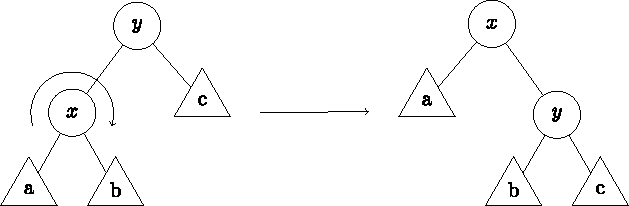
\includegraphics{images/zig.pdf}
    \label{fig:zig}

\caption{Caso zig com $x$ nó esquerdo da raiz.}
\end{figure}

\subsection{Caso zig-zig}

A rotação zig-zig acontece quando $x$ e seu pai são ambos filhos direitos ou ambos filhos esquerdos. Neste caso, é necessário rotacionar o pai de $x$ primeiro e em seguida rotacionar $x$.

\begin{figure}[h]
    \centering
    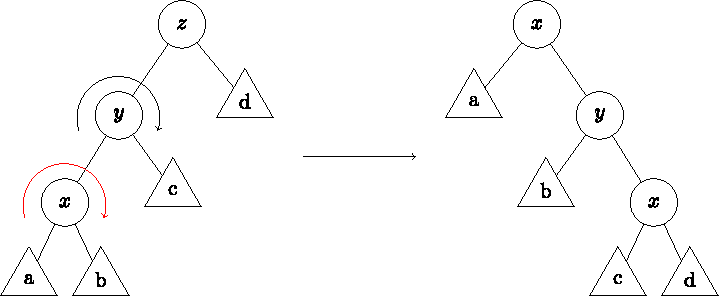
\includegraphics{images/zigzig.pdf}
    \label{fig:zigzig}

\caption{Caso zig-zig com $x$ e $y$ filhos esquerdos. A flecha preta e a vermelha representam respectivamente as rotações a serem realizadas em primeiro e por último.}
\end{figure}

\subsection{Caso zig-zag}

A rotação zig-zag acontece quando $x$ e seu pai não são ambos filhos direitos ou ambos filhos esquerdos. Neste caso, é necessário rotacionar $x$ duas vezes. Vale ressaltar que cada rotação será feita para um lado.
%\begin{figure}[hbt!]
%\centering
%\begin{tikzpicture}[
%ed/.style = {densely dashed, shorten >= 5pt},
%alpha/.style = {regular polygon, regular polygon sides=3, draw, minimum size=1.1cm, inner sep=2pt, anchor=south},
%level distance=1.5cm,
%sibling distance=0.25cm 
%]
%\begin{scope}[local bounding box=scope1]
%    \Tree [.$z$  [.$y$ \node[alpha]{a}; [.$x$ \node[alpha]{b}; \node[alpha]{c}; ]] \node[alpha]{d};]
%\end{scope}

%\begin{scope}[xshift=6cm, local bounding box=scope2, scale=1, level distance=2.25cm, sibling distance=0.25cm]
%    \Tree [.$x$ [.$y$ \node[alpha]{a}; \node[alpha]{b};] [.$z$  \node[alpha]{c}; \node[alpha]{d};]]]
%\end{scope}

%\draw[->] ([yshift=-0.5*\ht\strutbox,xshift=0.5cm]scope1.east) -- node {} ([yshift=-0.5*\ht\strutbox,xshift=-0.1cm]scope2.west); 

%\draw[->] ([yshift=-3.67cm, xshift=0.67cm]scope1.north) arc (-18:198:0.7cm);
%\draw[->,red] ([yshift=-3.67cm, xshift=-0.78cm]scope1.north) arc (198:-18:0.82cm);

%\end{tikzpicture}

\begin{figure}[h]
    \centering
    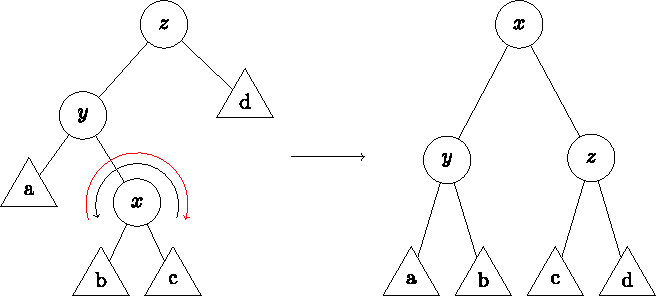
\includegraphics{images/zigzag.pdf}
    \label{fig:zigzag}

\caption{Caso zig-zag com $x$ filho direito e $y$ filho esquerdo. A flecha preta e a vermelha representam respectivamente as rotações a serem realizadas em primeiro e por último.}
\end{figure}

%%!TeX root=../tese.tex
%("dica" para o editor de texto: este arquivo é parte de um documento maior)
% para saber mais: https://tex.stackexchange.com/q/78101/183146

%% ------------------------------------------------------------------------- %%
\chapter{Conjectura da Otimalidade Dinâmica}
\label{cap:otimalidade-dinamica}

%!TeX root=../tese.tex
%("dica" para o editor de texto: este arquivo é parte de um documento maior)
% para saber mais: https://tex.stackexchange.com/q/78101/183146

%% ------------------------------------------------------------------------- %%
\chapter{Interpretação geométrica de buscas em ABBs}
\label{cap:geometria}

Neste capítulo iremos entender como interpretar de maneira geométrica os algoritmos de busca em ABBs.

\section{Visão geométrica de buscas}

Os algoritmos de busca dentro do modelo de computação adotado sempre iniciam o nó corrente na raiz da ABB e percorrem a árvore comparando a chave procurada com o nó corrente até encontrar o nó buscado.

Dada uma sequência $X = (x_{1},\ldots,x_{m})$ de $m$ acessos às chaves $x_{1}, x_{2},\ldots,x_{m}$, é possível ilustrar essa sequência $X$ de maneira gráfica em um plano cartesiano da seguinte forma: o eixo X representará as chaves armazenadas dentro da ABB e o eixo Y representará o tempo, ou seja, as buscas feitas nessa ABB. Assim, um ponto de coordenada ($x$,$y$) representa a busca da chave $x$ na ABB no instante de tempo $y$. Veja o exemplo da Figura~\ref{fig:geometria-inicial}.

\textit{Conjuntos arboreamente satisfeitos}: um par de pontos $(a,b)$ do conjunto $P$ é arboreamente satisfeito se $a$ e $b$ são ortogonalmente colineares ou se há pelo menos um ponto do conjunto \( P \setminus \{a,b\} \) que está dentro da área delimitada pelo retângulo de vértices $a$ e $b$. Um conjunto $P$ é arboreamente satisfeito se todos os pares de pontos do conjunto são arboreamente satisfeitos. Veja a Figura~\ref{fig:geometria-inicial}.

\begin{figure}[h!]
    \centering
    \begin{minipage}[b]{0.45\textwidth}
        \centering
        \begin{tikzpicture}[scale=0.8]
        \begin{axis}[
            xlabel={Chaves},
            ylabel={Buscas},
            grid=major,
            xmin=0, xmax=10,
            ymin=0, ymax=10,
            xtick={0,2,4,6,8,10},
            ytick={0,2,4,6,8,10}
        ]
        \addplot[only marks, mark=*] coordinates {
            (1,9)
            (2,2)
            (3,6)
            (4,10)
            (5,8)
            (6,4)
            (7,1)
            (8,7)
            (9,3)
            (10,5)
        };
        \end{axis}
        \end{tikzpicture}
    \end{minipage}\hfill
    \begin{minipage}[b]{0.45\textwidth}
        \centering
        \begin{tikzpicture}[scale=0.8]
        \begin{axis}[
            xlabel={Chaves},
            ylabel={Buscas},
            grid=major,
            xmin=0, xmax=10,
            ymin=0, ymax=10,
            xtick={0,2,4,6,8,10},
            ytick={0,2,4,6,8,10}
        ]
        \addplot[only marks, mark=*] coordinates {
            (1,9)
            (2,2)
            (3,6)
            (4,10)
            (5,8)
            (6,4)
            (7,1)
            (8,7)
            (9,3)
            (10,5)
        };

        \addplot[only marks, mark=*, red] coordinates {
            (2,1)
            (9,1)
            (2,3)
            (6,3)
            (7,3)
            (8,3)
            (6,5)
            (8,5)
            (9,5)
            (1,6)
            (2,6)
            (4,6)
            (5,6)
            (6,6)
            (8,6)
            (8,8)
            (4,9)
            (5,9)
        };
        \end{axis}
        \end{tikzpicture}
    \end{minipage}
    \caption{À esquerda, um gráfico representando a busca (7, 2, 9, 6, 10, 3, 8, 5, 1, 4). À direita, um gráfico representando a mesma busca porém com um conjunto arboreamente satisfeito de pontos.}
\label{fig:geometria-inicial}
\end{figure}

%Em um conjunto arboreamente satisfeito, todo par de pontos $(a,b)$ não ortogonalmente colineares que não possuiem  
%menor conjunto de pontos sempre tem dois em linha ou nas pontas pelo menos

Em um conjunto arboreamento satisfeito, todo par de pontos $(a,b)$ não ortogonalmente colineares, há sempre pelo menos um ponto de \( P \setminus \{a,b\} \) que está em alguma aresta que incide em $a$, e há também pelo menos um ponto que está em alguma aresta que incide em $b$.

% falta caption
\begin{center}
\begin{tikzpicture}
    \draw[blue, thick] (0,0) rectangle (2,1);
    
    \node at (0,0) [below left] {$a$};
    \node at (2,1) [above right] {$b$};
    
    \draw[red, thick] (0,0) -- (0,1);
    \draw[red, thick] (0,0) -- (2,0);
    \draw[blue, thick] (2,1) -- (0,1);
    \draw[blue, thick] (2,1) -- (2,0);
\end{tikzpicture}
\end{center}

\textbf{Prova:} Sejam $a$ e $b$ dois pontos de um conjunto arboreamente satisfeito. Como $(a,b)$ é um par de pontos arboreamente satisfeitos, então a área delimitada pelo retângulo de vértices $a$ e $b$ possui pelo menos 1 ponto diferente de $\{a,b\}$. Denotemos por $c$ tal ponto. Se $c$ não estiver em uma aresta que incide em $a$, então é possível recursivamente procurar tal ponto no par $(a,c)$ de pontos arboreamente satisfeitos. Analogamente, se $c$ não estiver em uma aresta que incide em $b$, então é possível recursivamente procurar tal ponto no par par $(c,b)$ de pontos arboreamente satisfeitos.

%Seja $\tau_i$ a subárvore // falar de subarvores?

A visão geométrica da execução de um algoritmo de busca em ABB para uma sequência $X = (x_{1},\ldots,x_{m})$ de buscas, de maneira similar, é o conjunto de pontos na forma ($x$,$y$) tal que $x$ foi uma chave acessada durante o instante de tempo $y$. É possível mapear esse conjunto de pontos para um plano cartesiano. Logo, todos os pontos com altura $y$ representam as chaves acessadas durante o instante de tempo $y$, ou seja, os nós acessados durante a busca por $x_y$. 
%não sei se eu gostei de $x_y$, porque $x$ é tanto coordenada quanto ponto na sequencia de busca

\textit{Lema 1.} A visão geométrica de qualquer execução de um algoritmo de busca em ABB no modelo de computação adotado é um conjunto de pontos arboreamente satisfeitos.

\textbf{Prova:} Assuma que a visão geométrica de um algoritmo de busca em ABB não é arboreamento satisfeita. Dessa maneira, há pelo menos um par de pontos $(a,b)$ nesse conjunto que não é arboreamente satisfeito. Seja $a$ a chave buscada no instante de tempo $i$ e seja $b$ a chave buscada no instante de tempo $j$. Assumiremos também sem perda de generalidade que $i < j$ e $a < b$.

Seja $c$ o ancestral comum mais profundo de $a$ e $b$ imediatamente antes da busca $i$. E seja $d$ o acestral comum mais profundo de $a$ e $b$ imediatamente antes da busca $j$.

Denotaremos números para áreas específicas para simplificar a explicação da prova. 
Área 1 = \{$(x,y)$ | $x = a$ e $i < y \leq j$\}, representando todos os acessos a $x$ entre os instantes de tempo $i$ e $j$. \\
Área 2 = \{$(x,y)$ | $a \leq x < b$ e $y = j$\}, representando todos os acessos a chaves entre $a$ e $b$ no instante de tempo $j$. \\
Área 3 = \{$(x,y)$ | $x = b$ e $i < y \leq j$\}, representando todos os acessos a $y$ entre os instantes de tempo $i$ e $j$. \\
Área 4 = \{$(x,y)$ | $a \leq x < b$ e $y = j$\}, representando todos os acessos a chaves entre $a$ e $b$ no instante de tempo $i$. \\
%Área 5 = \{$(x,y)$ | $a \leq x < b$ e $y = j$\}, representando todos os acessos a chaves entre $a$ e $b$ no instante de tempo $i$. \\

Como $(a,b)$ não são arboreamente satisfeitos, nota-se que não há nenhum ponto tanto nas bordas quanto no interior do retângulo de vértices $a$ e $b$. Logo $1 \cup 2 \cup 3 \cup 4 = \emptyset$.

\begin{figure}[H]
    \centering
    \begin{minipage}[t]{0.70\textwidth}
        Se $2 = \emptyset$, então $d = y$. Porém, se $d = y$ então, pelo menos em algum outro instante de tempo $h$, $h < j$, $y$ também era o ancestral comum mais profundo entre $a$ e $b$, logo $3 \neq \emptyset$. Por contrapositiva, se $3 = \emptyset \Rightarrow 2 \neq \emptyset$.

        Por $c$ ser o ancestral comum mais profundo de $a$ e $b$ no instante $i$, sabemos que $x \leq c \leq y$ e mais importante, $c$ está mais acima na ABB. Logo, para acessar qualquer chave no intervalo $[a,b]$, no instante $i$, é preciso acessar a chave $c$.
        
        Se $4 = \emptyset$, então $c = x$. Porém $b$ é acessado no instante $j$. Se $c = d$, $a$ precisa ser acessados no instante de tempo $j$, logo $1 \neq \emptyset$. Caso $c \neq d$, então em algum instante de tempo $h$, $i \leq h < j$, o ancestral comum mais profundo entre $a$ e $b$ mudou, logo algum nó com chave no intervalo $(a,b]$ precisa ter sido rotacionado para cima, porém de acordo com o modelo de computação só é possível rotacionar um nó depois de acessa-lo e sabemos que qualquer acesso no intervalo $[a,b]$ no instante de tempo $h$, precisa acessar o ancestral comum mais profundo que neste caso é $x$. Logo $1 \neq \emptyset$. Por contrapositiva, $1 = \emptyset \Rightarrow 4 \neq \emptyset$.

    \end{minipage}\hfill
    \begin{minipage}[t]{0.25\textwidth}
        % Coluna da direita com a imagem
        \centering
        \begin{adjustbox}{valign=t} % Alinha o gráfico ao topo da caixa
        \begin{tikzpicture}[scale=0.6]
        \begin{axis}[
            xlabel={Chaves},
            ylabel={Buscas},
            grid=major,
            xmin=0, xmax=3,
            ymin=0, ymax=3,
            xtick={1,2},
            ytick={1,2},
            xticklabels={a,b}, % Define os rótulos do eixo x
            yticklabels={i,j} % Define os rótulos do eixo y
        ]

        \addplot[only marks, mark=*] coordinates {
            (1,1)
            (2,2)
        };

        \addplot[red, thick] coordinates {
            (1,2)
            (2,2)
        };

        \addplot[red, thick] coordinates {
            (2,2)
            (2,1)
        };

        \addplot[red, thick] coordinates {
            (1,1)
            (1,2)
        };

        \addplot[red, thick] coordinates {
            (1,1)
            (2,1)
        };

        % Adiciona rótulos aos pontos
        \node at (axis cs:1,1) [anchor=north east, fill=white, font=\small] {$a$};
        \node at (axis cs:2,2) [anchor=south west, fill=white, font=\small] {$b$};

        \node at (axis cs:1,1.5) [anchor=east, font=\normalsize] {1};
        \node at (axis cs:1.5,2) [anchor=south, font=\normalsize] {2};
        \node at (axis cs:2,1.5) [anchor=west, font=\normalsize] {3};
        \node at (axis cs:1.5,1) [anchor=north, font=\normalsize] {4};
        %\node at (axis cs:1.5,1.5) [anchor=center, font=\normalsize] {5};

        \end{axis}
        \end{tikzpicture}
        \end{adjustbox}
    \end{minipage}
    %\caption{Gráfico de chaves e buscas}
    \label{fig:chaves-buscas}
\end{figure}

Lema 2. Qualquer conjunto de pontos arboreamente satisfeitos representa a execução de um algoritmo de busca em ABB no modelo de computação adotado.
%!TeX root=../tese.tex
%("dica" para o editor de texto: este arquivo é parte de um documento maior)
% para saber mais: https://tex.stackexchange.com/q/78101/183146

%% ------------------------------------------------------------------------- %%
\chapter{Algoritmo Guloso}
\label{cap:algoritmo-guloso}



%%%%%%%%%%%%%%%%%%%%%%%%%%%% APÊNDICES E ANEXOS %%%%%%%%%%%%%%%%%%%%%%%%%%%%%%%%

% Um apêndice é algum conteúdo adicional de sua autoria que faz parte e
% colabora com a ideia geral do texto mas que, por alguma razão, não precisa
% fazer parte da sequência do discurso; por exemplo, a demonstração de um
% teorema intermediário, as perguntas usadas em uma pesquisa qualitativa etc.
%
% Um anexo é um documento que não faz parte da tese (em geral, nem é de sua
% autoria) mas é relevante para o conteúdo; por exemplo, a especificação do
% padrão técnico ou a legislação que o trabalho discute, um artigo de jornal
% apresentando a percepção do público sobre o tema da tese etc.
%
% Os comandos appendix e annex reiniciam a numeração de capítulos e passam
% a numerá-los com letras. "annex" não faz parte de nenhuma classe padrão,
% foi criado para este modelo. Se o trabalho não tiver apêndices ou anexos,
% remova estas linhas.
%
% Diferentemente de \mainmatter, \backmatter etc., \appendix e \annex não
% forçam o início de uma nova página. Em geral isso não é importante, pois
% o comando seguinte costuma ser "\chapter", mas pode causar problemas com
% a formatação dos cabeçalhos. Assim, vamos forçar uma nova página antes
% de cada um deles.

%%%% Apêndices %%%%

%\cleardoublepage

%\pagestyle{appendix}

%\appendix

% \addappheadtotoc acrescenta a palavra "Apêndice" ao sumário; se
% só há apêndices, sem anexos, provavelmente não é necessário.
%\addappheadtotoc

%\input{conteudo/apendice-exemplo-faq}
%\par

%%%% Anexos %%%%

%\cleardoublepage

%\pagestyle{appendix} % repete o anterior, caso você não use apêndices

%\annex

% \addappheadtotoc acrescenta a palavra "Anexo" ao sumário; se
% só há anexos, sem apêndices, provavelmente não é necessário.
%\addappheadtotoc

%\input{conteudo/anexo-exemplo-imegoodies}
%\par
%\input{conteudo/anexo-exemplo-pseudocodigo}
%\par


%%%%%%%%%%%%%%% SEÇÕES FINAIS (BIBLIOGRAFIA E ÍNDICE REMISSIVO) %%%%%%%%%%%%%%%%

% O comando backmatter desabilita a numeração de capítulos.
\backmatter

\pagestyle{backmatter}

% Espaço adicional no sumário antes das referências / índice remissivo
%\addtocontents{toc}{\vspace{2\baselineskip plus .5\baselineskip minus .5\baselineskip}}

% A bibliografia é obrigatória

\printbibliography[
  %title=\refname\label{sec:bib}, % "Referências", recomendado pela ABNT
  title=\bibname\label{sec:bib}, % "Bibliografia"
  heading=bibintoc, % Inclui a bibliografia no sumário
]

%\printindex % imprime o índice remissivo no documento (opcional)

\end{document}